% This must be in the first 5 lines to tell arXiv to use pdfLaTeX, which is strongly recommended.
\pdfoutput=1
% In particular, the hyperref package requires pdfLaTeX in order to break URLs across lines.

\documentclass[11pt]{article}

% Remove the "review" option to generate the final version.
\usepackage{ACL2023}

% Standard package includes
\usepackage{times}
\usepackage{latexsym}

% For proper rendering and hyphenation of words containing Latin characters (including in bib files)
\usepackage[T1]{fontenc}
% For Vietnamese characters
% \usepackage[T5]{fontenc}
% See https://www.latex-project.org/help/documentation/encguide.pdf for other character sets

% This assumes your files are encoded as UTF8
\usepackage[utf8]{inputenc}

% This is not strictly necessary, and may be commented out.
% However, it will improve the layout of the manuscript,
% and will typically save some space.
\usepackage{microtype}

% This is also not strictly necessary, and may be commented out.
% However, it will improve the aesthetics of text in
% the typewriter font.
\usepackage{inconsolata}

\usepackage{amsmath}
\usepackage{amsfonts}
\usepackage{mathtools}

\usepackage{todonotes}

\newtheorem{hyp}{Hypothesis}

% If the title and author information does not fit in the area allocated, uncomment the following
%
%\setlength\titlebox{<dim>}
%
% and set <dim> to something 5cm or larger.

\title{Consistency text similarity on the example of the task of recognizing hallucinations of language models}

% Author information can be set in various styles:
% For several authors from the same institution:
% \author{Author 1 \and ... \and Author n \\
%         Address line \\ ... \\ Address line}
% if the names do not fit well on one line use
%         Author 1 \\ {\bf Author 2} \\ ... \\ {\bf Author n} \\
% For authors from different institutions:
% \author{Author 1 \\ Address line \\  ... \\ Address line
%         \And  ... \And
%         Author n \\ Address line \\ ... \\ Address line}
% To start a seperate ``row'' of authors use \AND, as in
% \author{Author 1 \\ Address line \\  ... \\ Address line
%         \AND
%         Author 2 \\ Address line \\ ... \\ Address line \And
%         Author 3 \\ Address line \\ ... \\ Address line}

\author{Kseniia Petrushina \\
  % Affiliation / Address line 1 \\
  \texttt{petrushina.ke@phystech.edu}}

\begin{document}
\maketitle
\begin{abstract}

This work explores the recognition of hallucinations of language models in the tasks of machine translation, paraphrasing and modeling definitions. Approaches to solving this problem are based on measures of semantic similarity between sentences. We compare different approaches to the solution, and also propose a new measure of proximity - \textit{consistency similarity}.

\end{abstract}

\section{Introduction}

Currently, there is a real boom in language models that are able to perform various tasks of Natural Language Generation (NLG).

A hallucination of the language model is a grammatically correctly generated response, which, however, contains incorrect information. And currently, language models apt to give a fluent answer, in particular due to the fact that they adjusted to metrics that pay attention to the sonority of the answer, rather than its factual component. In the tasks of paraphrasing and machine translation, hallucination is different meanings in the generated and original sentences. Also, hallucinations may be discrepancies between the model's response and the actual data from the external knowledge base.

\section{Problem statement}

\textit{Language model} is a function 
\[\mathbf{f}: \mathcal{P}(\mathbf{T_s}^{L_s})\to \mathcal{P}(\mathbf{T_h}^{L_h}),\]
where $\mathbf{s} \in \mathbf{T_s}^{L_s}$ is a sequence of $L_s$ tokens from the overall set of source tokens $\mathbf{T_s}$, $\mathbf{h} \in \mathbf{T_h}^{L_h}$ is a sequence of $L_h$ tokens from the overall set of hypothesis tokens $\mathbf{T_h}$. And $\mathcal{P}(\mathbf{T}^{L})$ is the probability distribution over $\mathbf{T}^{L}$. $\mathbf{s}_i$ is called \textit{source sentence} and $\mathbf{h}_i$ is called \textit{model hypothesis}.

Assuming $\mathbf{f}$ has the following output probabilities \[\mathcal{P}(\mathbf{f}(\mathbf{s}) = \mathbf{h}) = p_{\mathbf{sh}}\]
we can define function \[\mathbf{f}^{-1}: \mathcal{P}(\mathbf{T_h}^{L_h}) \to \mathcal{P}(\mathbf{T_s}^{L_s})\]
Then it is said that $\mathbf{h} = \mathbf{f}(\mathbf{s})$ is a \textit{hallucination} of the language model $\mathbf{f}$ with the input $\mathbf{s}$ if \[p(\mathbf{f}^{-1}(\mathbf{f}(\mathbf{s})) = \mathbf{s}) = 0.\] This is illustrated in the Figure \ref{fig:hal}.

\begin{figure}
    \centering
    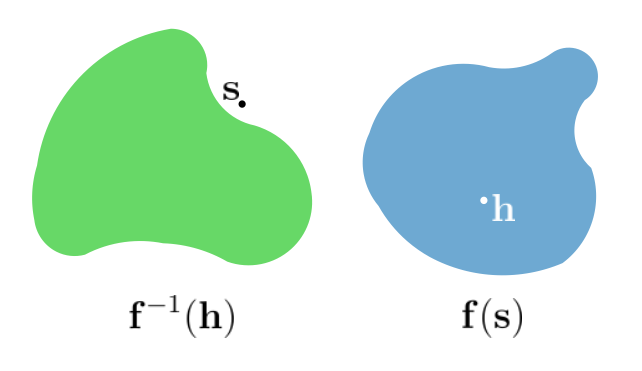
\includegraphics[width=0.4\textwidth]{images/hallucination.png}
    \caption{An illustration of a model's hallucination. $\mathbf{s}$ does not belong to the set of possible outputs of $\mathbf{f}^{-1}(\mathbf{h})$}
    \label{fig:hal}
\end{figure}

The task of recognizing hallucinations is to find a function $sim: \mathbf{T_s}^{L_s} \times \mathbf{T_h}^{L_h} \to [0, 1]$, such that
\[\mathbb{E}_{\mathbf{s}_i \sim \mathbf{T_s}^{L_s}, \mathbf{h}_i \sim f(\mathbf{s}_i)} \{\mathbb{I}[sim(\mathbf{s}_i, \mathbf{h}_i) \ge \text{thr}] = y_i \} \to \max\limits_{sim, \text{thr}},\]
where $y_i$ denotes the presence of a hallucination.

The function $sim(\mathbf{s}, \mathbf{h})$ is perceived as similarity measure between source sentence $\mathbf{s}$ and model hypothesis $\mathbf{h}$.

\section{Theory}

\subsection{Existing solutions}

The tasks of paraphrasing and textual style transfer rely on measuring similarity between sentences \cite{babakov-etal-2022-large}. This is done using different functions $sim: \mathbf{T_s}^{L_s} \times \mathbf{T_h}^{L_h} \to [0, 1]$.

These content preserving metrics can be divided into the following groups:

\textbf{Words or characters n-grams} The similarity of the sentences can be calculated based on n-gramms, i.e. all possible subsequences of $\mathbf{s}$ and $\mathbf{h}$ of length $n$. \[N_{s} \subset \mathbf{T_s}^{n}, \quad N_{h} \subset \mathbf{T_h}^{n} \]
\[sim_\text{BLEU}(\mathbf{s}, \mathbf{h}) = \frac{|N_{s} \cap N_{h}|}{|N_{h}|}\]

\textbf{Similarity between static embeddings} A vector space $\mathbb{R}^d$ can be a more convenient representation of the text for calculating distances. So, the $\mathbf{emb}: \mathbf{T_s} \cup \mathbf{T_h} \to \mathbb{R}^d$ function is introduced. Vector from the sentence $\mathbf{s}$ will be obtained according to the following formula: \[\mathbf{v_s} = \dfrac{1}{L_s} \sum\limits_{i=1}^{L_s} \mathbf{emb} (\mathbf{s}[i]) \]
Then the similarity is: \[sim_\text{cos}(\mathbf{s}, \mathbf{h}) = \cos (\mathbf{v_s}, \mathbf{v_h})\]

\textbf{Similarity between contextualized embeddings} Vector representation of a token can depend on the context, i.e. surrounding tokens. Contextualized embeddings are obtained using model $\mathbf{enc}: \mathbf{T_s}^{L_s} \to \mathbb{R}^{L_s \times d}$. $\mathbf{v_s} = \{v_1, \dots, v_{L_s}\}$, $\mathbf{v_h} = \{\hat{v}_1, \dots, \hat{v}_{L_h}\}$. BERTScore \cite{zhang-bertscore} is calculated as \[R = \dfrac{1}{L_s} \sum\limits_{v_i \in \mathbf{v_s}} \max\limits_{\hat{v}_j \in \mathbf{v_h}} v^T_i \hat{v}_j \; P = \dfrac{1}{L_h} \sum\limits_{\hat{v}_j \in \mathbf{v_h}} \max\limits_{v_i \in \mathbf{v_s}} v^T_i \hat{v}_j \] 
\[\text{BERTScore} = 2\dfrac{P R}{P + R}\]

\textbf{Similarity between embeddings from bi-encoders} Encoder models $\mathbf{enc_s}: \mathbf{T_s}^{L_s} \to \mathbb{R}^d$, $\mathbf{enc_h}: \mathbf{T_h}^{L_h} \to \mathbb{R}^d$ implicitly get a vector representations of the entire sentences. The resulting similarity can be calculated as \[sim_\text{bi-enc}(\mathbf{s}, \mathbf{h}) = \cos (\mathbf{enc_s}(\mathbf{s}), \mathbf{enc_h}(\mathbf{h}))\]
An example of such encoder model is LaBSE \cite{feng-etal-2022-language}.

\textbf{Symmetric and asymmetric cross-encoders} Encoder model $\mathbf{enc}: \mathbf{T_s}^{L_s} \times \mathbf{T_h}^{L_h} \to \mathbb{R}^d$, uses cross-attention mechanism \cite{vaswani-attention} when processing two texts at the same time. It is symmetrical if $\mathbf{enc}(\mathbf{s}, \mathbf{h}) = \mathbf{enc}(\mathbf{h}, \mathbf{s})$, otherwise it is asymmetrical, this property is determined by the NLG problem being solved. The $\mathbf{clf}: \mathbb{R}^d \to [0, 1]$ function is also introduced, which determines the value of the similarity measure. \[sim_\text{cross-enc}(\mathbf{s}, \mathbf{h}) = \mathbf{clf}(\mathbf{enc}(\mathbf{s}, \mathbf{h}))\]

\subsection{Proposed method}

First, in the general case, the similarity function should be defined for objects from different spaces $\mathbf{T_s}^{L_s}$ and $\mathbf{T_h}^{L_h}$. Secondly, the existing methods do not investigate whether there is enough information in $\mathbf{h}$ to restore $\mathbf{s}$. Therefore, we suggest using a new metric - \textit{consistency similarity measure}.

Consistency similarity measure is defined by
\[{sim}_{\mathbf{C}} (\mathbf{s}_i, \mathbf{h}_i) = {sim}(\mathbf{s}_i, \mathbf{f}^{-1}(\mathbf{h}_i))),\]
where ${sim}$ can be arbitrary method from the existing solutions.

The benefits of the proposed formula are:

\begin{enumerate}
    \item The arguments of the function lie in the same space $\mathbf{T_S}^{L_s}$.
    \item This similarity measure depends on how well the information about $\mathbf{s}_i$ is preserved in $\mathbf{h}_i$ and what the model $\mathbf{f}^{-1}$ can restore:
    \begin{hyp}
    \[\mathbb{E}_{\mathbf{f}^{-1}(\mathbf{h}_i)} {sim}_{\mathbf{C}} (\mathbf{s}_i, \mathbf{h}_i) \le{sim} (\mathbf{s}_i, \mathbf{h}_i) \]
    \end{hyp}
\end{enumerate}

\begin{hyp}
Consistency similarity measure $sim_\text{C}$ will be more stable and will give higher accuracy values.
\end{hyp}

\section{Computational experiments}

\subsection{Data}

We are given the dataset
\[\mathcal{D} = \{(\mathbf{s}_i, \mathbf{h}_i, y_i) \}_{i=1}^N, \quad \mathbf{h}_i \in \mathbf{f}(\mathbf{s}_i).\]

The target variable $y_i \in \{0, 1\}$ defines a binary relation on the subset of the set $\mathbf{T_s}^{L_s} \times \mathbf{T_h}^{L_h}$ represented in $\mathcal{D}$ and, in our formulation, it indicates the occurrence of a hallucination in the $\mathbf{f}$ model at the input of $\mathbf{s}_i$ and the output of $\mathbf{h}_i$.

\subsection{Metrics}

Given similarity predictions $\hat{y}_i = sim(\mathbf{s}_i, \mathbf{h}_i)$ the quality metrics in the hallucination recognition task are 

\begin{enumerate}
    \item The proportion of correct predictions:
    \[\text{Accuracy} = \frac1N \sum\limits_{i=1}^N \mathbb{I}[\hat{y}_i \ge \text{thr}] = y_i\]
    \item Spearman's rank correlation coefficient:
    \[r_s= \rho_{R(Y), R(\hat{Y})} = \frac{\text{cov} (R(Y), R(\hat{Y}))}{\sigma_{R(Y)} \sigma_{R(\hat{Y})}}\]
\end{enumerate}

\subsection{Paraphrase generation}

The detection of hallucinations in the paraphrase generation (PG) task assumes that the sentences $\mathbf{s}_i,~\mathbf{h}_i$ are in the same space $\mathbf{T}^{N}$. 

The results of the experiments are presented in the Table \ref{tab:pg}. $sim_\text{bi-enc}$ uses the Sentence Transformer \cite{reimers-gurevych-2019-sentence} as a text encoder. Consistency similarity $sim_\text{C}$ is calculated like $sim_\text{bi-enc} (\mathbf{s}_i, \mathbf{f}^{-1} (\mathbf{h}_i))$, since in the task of paraphrasing $\mathbf{f}^{-1} \equiv \mathbf{f}$.

\begin{table}[]
    \centering
    \begin{tabular}{c|c c}
    Method & Accuracy $\uparrow$ & $r_s \uparrow$ \\
    \hline
    $sim_\text{bi-enc}$ & 0.808 & 0.153 \\
    $sim_\text{C}$ & \textbf{0.824} & \textbf{0.186} \\
    \end{tabular}
    \caption{Hallucination recognition results in the PG task}
    \label{tab:pg}
\end{table}

\subsection{Machine translation}

In the machine translation (MT) task, texts are written in various languages. In this problem, $\mathbf{s}_i$ is in Russian and $\mathbf{h}_i$ is in English.

The results of the experiments are presented in the Table \ref{tab:mt}. The considered methods also use bi-encoders, vector representations are obtained using LaBSE and SONAR \cite{Duquenne2023SONARSM} models. SONAR embeddings subsequently are processed with BLASER model. \[sim_\text{LaBSE} = cos (\mathbf{enc}_{L}(\mathbf{s}_i), \mathbf{enc}_{L}(\mathbf{h}_i))\] 
\[sim_\text{BLASER-QE} = \mathbf{clf}_\text{B} (\mathbf{enc}_{S}(\mathbf{s}_i), \mathbf{enc}_{S}(\mathbf{h}_i))\]

\begin{table}[]
    \centering
    \begin{tabular}{c|c c}
    Method & Accuracy $\uparrow$ & $r_s \uparrow$ \\
    \hline
    $sim_\text{LaBSE}$ & 0.786 & 0.592 \\
    $sim_\text{BLASER-QE}$ & \textbf{0.802} & \textbf{0.605} \\
    \end{tabular}
    \caption{Hallucination recognition results in the MT task}
    \label{tab:mt}
\end{table}

% \subsection{Definition modeling}

% In the definition modeling (DM) task, the model $\mathbf{f}$ must predict the meaning of a word $\mathbf{w}$ - subsequence of $\mathbf{s}_i$. The text $\mathbf{s}_i$ represents the use of the word of interest $\mathbf{w}$ in the context and $\mathbf{h}_i$ is a generated definition. This task can be reduced to exploring the similarity between sentences as follows: the retriever function $\mathbf{r}$ is introduced, which returns the definition of a word $\mathbf{w}$ using an external database. Then the detection of the hallucination of the model $\mathbf{f}$ when performing the DM task can be reformulated as calculating $sim(\mathbf{r}(\mathbf{w}), \mathbf{h}_i)$.

% The results of the experiments are presented in the Table \ref{tab:dm}. The definitions of the words were obtained using the RAG-Token Model \cite{rag2020} and parsed from Wiktionary. The obtained definitions $\mathbf{r}_\text{RAG}(\mathbf{w})$ were compared with $\mathbf{h}_i$ using Sentence Transformer. And for Wiktionary definitions we used E5 encoder model \cite{wang2022text}.

% \begin{table}[]
%     \centering
%     \begin{tabular}{c|c c}
%     Method & Accuracy $\uparrow$ & $r_s \uparrow$ \\
%     \hline
%     $sim_\text{RAG}$ & 0.593 & - \\
%     $sim_\text{Wiki}$ & \textbf{0.653} & - \\
%     \end{tabular}
%     \caption{Hallucination recognition results in the DM task}
%     \label{tab:dm}
% \end{table}

\section{Conclusion}
We conducted a review of existing methods for investigating the proximity between two texts, and also proposed a new method - consistency similarity, which draws attention to the correspondence of the semantic content of model hypothesis to information in source sentence. 

\bibliography{anthology,custom}
\bibliographystyle{acl_natbib}

\appendix

% \section{Appendix}
% \label{sec:appendix}


\end{document}
